\documentclass[11pt, addpoints, answers]{exam}

\usepackage{amsmath, amssymb}
\usepackage{xcolor}
\usepackage{tikz}
\usepackage{enumerate}
\usepackage{graphicx}
\usepackage{tabularx}

\newcommand{\red}[1]{\textcolor{red}{#1}}
\newcommand{\blue}[1]{\textcolor{blue}{#1}}
% For inserting code snippets.
\usepackage{listings}
\lstset{
    columns = fixed,
    basewidth = {0.5em},
    breaklines = true,
    backgroundcolor = \color{white},
    keywordstyle = \color[RGB]{40, 40, 255},
    numberstyle = \footnotesize\color{darkgray},
    commentstyle = \ttfamily\color{violet},
    basicstyle = \ttfamily,
    stringstyle = \ttfamily\color[RGB]{128, 0, 0},
    showstringspaces = false,
    language = {[11]C++},
    escapechar = \@
}
\lstnewenvironment{cpp}[1][]{\lstset{language = {[11]C++}, #1}}{}

\renewcommand{\baselinestretch}{1.15}
\setlength{\parskip}{1.25\baselineskip}

% headers, footers, titles
\newcommand{\CourseName}{CS101 Algorithms and Data Structures}
\newcommand{\HomeworkNO}{7}
\newcommand{\DueDate}{November 20, 2024} % TODO: REMEMBER TO MODIFY

\pagestyle{headandfoot}
\runningheadrule
\runningheader{CS101 24Fall}{Homework \HomeworkNO}{Due on: \DueDate}
\runningfooter{}{\thepage}{}

\title{
    \vspace{25pt}
    \LARGE ShanghaiTech University \\
    \bigskip
    \textbf{\CourseName} \\
    \textbf{Fall 2024}   \\
    \bigskip
    Homework \HomeworkNO
}
\author{}
\date{Due date: \DueDate, at 23:59}

% formats of questions, choices, points, etc.
\qformat{\bf\thequestion. (\totalpoints\ points) \thequestiontitle\hfill}
\pointname{'}
\SolutionEmphasis{\color{black}}
\CorrectChoiceEmphasis{\bf\color{blue}}



% We frequently use this font.
\newcommand{\dfuttt}{\texttt}
\newcommand{\bluett}[1]{\textcolor{blue}{\ttt{#1}}}

% \newif\ifprintanswers
% \printanswersfalse

\begin{document}

\maketitle

\vspace{50pt}

\begin{enumerate}
    \item Please write your solutions in English.
    \item Submit your solutions to Gradescope.
    \item Set your FULL name to your Chinese name and your STUDENT ID correctly in Gradescope account settings.
    \item If you want to submit a handwritten version, scan it clearly. CamScanner is recommended.
    \item When submitting, match your solutions to the problems correctly.
    \item No late submission will be accepted.
    \item Violations to any of the above may result in zero points.
\end{enumerate}

\newpage

\begin{questions}

\titledquestion{Multiple Choices}

Each question has \textbf{one or more} correct answer(s). Select all the correct answer(s). For each question, you will get 0 points if you select one or more wrong answers, but you will get half points if you select a non-empty subset of the correct answers.

Write your answers in the following table.

%%%%%%%%%%%%%%%%%%%%%%%%%%%%%%%%%%%%%%%%%%%%%%%%%%%%%%%%%%%%%%%%%%%%%%%%%%%
% Note: The `LaTeX' way to answer a multiple-choices question is to replace `\choice'
% with `\choice', as what you did in the first question. However, there are still
% many students who would like to handwrite their homework. To make TA's work easier,
% you have to fill your selected choices in the table below, no matter whether you use 
% LaTeX or not.
%%%%%%%%%%%%%%%%%%%%%%%%%%%%%%%%%%%%%%%%%%%%%%%%%%%%%%%%%%%%%%%%%%%%%%%%%%%

\begin{table}[h]
    \centering
    \renewcommand{\arraystretch}{1.25}
    \begin{tabular}{|p{2cm}|p{2cm}|p{2cm}|p{2cm}|p{2cm}|p{2cm}|}
        \hline 
        (a) & (b) & (c) & (d) & (e) & (f) \\
        \hline
        % YOUR ANSWER HERE.
        &  &  &  &  &  \\

        \hline
    \end{tabular} 
\end{table}

\begin{parts}

    \part[2] Consider a table of capacity 11 using open addressing with hash function \( k \bmod 11\) and linear probing. After inserting 7 values into an empty hash table, the table is below. Which of the following choices give a possible order of the key insertion sequence?
    
    \begin{table}[h]
        \centering
        \begin{tabular}{|c|l|l|l|l|l|l|l|l|l|l|l|}
            \hline
            Index & 0 & 1 & 2 & 3 & 4  & 5  & 6 & 7 & 8 & 9 & 10\\
            \hline
            Keys  &  &  & 24 & 47 & 26  & 3 & 61 & 15 & 49 & & \\
            \hline
        \end{tabular}
    \end{table}
    
    \begin{choices}
        \choice 26, 61, 47, 3, 15, 24, 49
        \choice 26, 24, 3, 15, 61, 47, 49
        \choice 24, 61, 26, 47, 3, 15, 49
        \choice 26, 61, 15, 49, 24, 47, 3
    \end{choices}
    
    \part[2] Consider a table of capacity 8 using open addressing with hash function \( h(k) = k \bmod 8\) and probing function $H(k) = h(k) + c_1i + c_2i^2\mod 8$ with $c_1=c_2=0.5$. After inserting 7 values into an empty hash table, the table is below. Which of the following choices give a possible order of the key insertion sequence?
    \begin{table}[h]
        \centering
        \begin{tabular}{|c|l|l|l|l|l|l|l|l|l|l|l|}
            \hline
            Index & 0 & 1 & 2  & 3  & 4  & 5  & 6  & 7 \\
            \hline
            Keys  & 14 & 6 & 10 & 9 & 25 &   & 22 & 15 \\
            \hline
        \end{tabular}
    \end{table}
    \begin{choices}
        \choice 15, 22, 10, 6, 25, 14, 9
        \choice 10, 22, 15, 6, 14, 9, 25
        \choice 6, 25, 15, 14, 22, 9, 10
        \choice 10, 22, 15, 6, 14, 9, 25
    \end{choices}
    
    \part[2] Which of the following statements about the hash table are true?
    \begin{choices}
        \choice We have a hash table of size \(2n\) with a uniformly distributed hash function. If we store \(n\) elements into the hash table, then with a very high probability, there will be \textbf{no} hash collision.
        \choice In a hash table with a uniformly distributed hash function where collisions are resolved by chaining, an unsuccessful search (i.e. the required element does not exist in the table) takes \(\Theta(1)\) on average if the load factor of the hash table is \(O(1)\).
        \choice Lazy erasing means marking the entry/bin as erased rather than deleting it.
        \choice Rehashing is a technique used to resolve hash collisions.
    \end{choices}
    
    
    \part[2] Applying insertion sort and the most basic bubble sort without a flag respectively on the same array, for both algorithms, which of the following statements is/are true? (simply assume we are using swapping for insertion sort)
    \begin{choices}
        \choice There are two for-loops, which are nested within each other.
        \choice They need the same amount of element comparisons.
        \choice They need the same amount of swaps.
        \choice None of the above.
    \end{choices}
    
    \part[2] In the lecture we have learned that different sorting algorithms are suitable for different scenarios. Which of the following statements is/are suitable for insertion sort?
    \begin{choices}
        \choice Each element of the array is close to its final sorted position.
        \choice An array where only a few elements are not in its final sorted position.
        \choice A big sorted array with a small sorted array concatenated to it.
        \choice None of the above.
    \end{choices}
    
    \part[2] The time complexity for both insertion sort and bubble sort will be the same if: (assume bubble sort is flagged bubble sort)
    \begin{choices}
        \choice the input array is reversely sorted.
        \choice the input array is a list containing n copies of the same number.
        \choice the input array is already sorted.
        \choice None of the above.
    \end{choices}

\end{parts}

\titledquestion{Disjoint Set Practice}

Given the following set of operations on a disjoint set(initially there are six disjoint elements), show the final disjoint set tree for each of the following optimization strategies:

\begin{itemize}
    \item $set\_union(A, B)$
    \item $set\_union(C, D)$
    \item $set\_union(B, C)$
    \item $find(D)$
    \item $set\_union(E, F)$
    \item $set\_union(E, A)$
\end{itemize}

\begin{parts}
    \part[5] Only with union-by-rank optimization. (When two trees have the same height, the set specified first in the union will be the root of the merged set.)
    \begin{solution}
        \vspace{100pt}
    \end{solution}
    \part[5] Only with path compression. (The set specified first in the union will always be the root of the merged set.)
    \begin{solution}
        \vspace{100pt}
    \end{solution}
\end{parts}


\titledquestion{Graph traversal}
Consider the following directed graph starting with A.

\centering
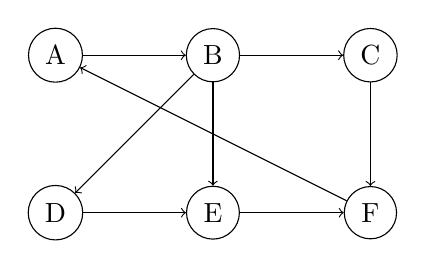
\begin{tikzpicture}[node distance=2cm]
    \node[circle, draw] (A) {A};
    \node[circle, draw, right of=A] (B) {B};
    \node[circle, draw, right of=B] (C) {C};
    \node[circle, draw, below of=A] (D) {D};
    \node[circle, draw, right of=D] (E) {E};
    \node[circle, draw, right of=E] (F) {F};

    \draw[->] (A) -- (B);
    \draw[->] (B) -- (C);
    \draw[->] (B) -- (D);
    \draw[->] (B) -- (E);
    \draw[->] (C) -- (F);
    \draw[->] (D) -- (E);
    \draw[->] (E) -- (F);
    \draw[->] (F) -- (A);
\end{tikzpicture}

\begin{parts}

\part[3]  Give the adjacency list for the graph. You should write the node in alphabetical order. (Leave it blank if the node has no neighbour)

\begin{align*} % Your solution here
    adj(A) =& [\underline{\qquad\qquad}],\\
    adj(B) =& [\underline{\qquad\qquad}],\\
    adj(C) =& [\underline{\qquad\qquad}],\\
    adj(D) =& [\underline{\qquad\qquad}],\\
    adj(E) =& [\underline{\qquad\qquad}],\\
    adj(F) =& [\underline{\qquad\qquad}],\\
\end{align*}


\part[3] Give the visited node order using the above adjacency list for Breadth First Search.
\begin{solution}
    
\end{solution}

\part[3] Give the visited node order using the above adjacency list for Depth First Search.
\begin{solution}
    
\end{solution}

\end{parts}

\raggedright
\titledquestion{DFS went wrong!}[6]
The following algorithm which runs DFS on a directed graph, but it contains a fatal error.
\begin{lstlisting}
    Create a stack.
    Choose the initial vertex and mark it as visited.
    Put the initial vertex onto the stack.
    while the stack is not empty:
        Pop a vertex V from the top of the stack.
        for each neighbor of V:
            if that neighbor is not marked as visited:
                Mark that neighbor as visited.
                Push that neighbor onto the stack.
\end{lstlisting}

    
Please give a graph as an counterexample and briefly explain why this algorithm is wrong. 
\\
\textit{Note: In this problem, we say a node is ``visited" whenever it is marked as visited. Pay special attention to how this method differs from the standard DFS in terms of the order in which nodes are marked as visited.}\\


\raggedright
\begin{solution}
    \vspace{200pt}
\end{solution}

\titledquestion{Friend or enemy?}[6]
\raggedright
Consider a set of \( n \) individuals, each of whom can have two types of relationships with others: friendship and enmity. It is also possible for individuals to have no relationship at all, or even to be both friends and enemies simultaneously. The relationships satisfy the following properties:

\begin{enumerate}
    \item If person \( a_i \) is a friend of person \( a_j \), then person \( a_j \) is also a friend of person \( a_i \) (friendship is symmetric).
    \item If person \( a_i \) is an enemy of person \( a_j \), then person \( a_j \) is also an enemy of person \( a_i \) (enmity is symmetric).
    \item Friends of friends are also considered friends. That is, if person \( a_i \) is a friend of person \( a_j \) and person \( a_j \) is a friend with person \( a_k \), then person \( a_i \) is a friend of person \( a_k \).
    \item Enemies of enemies are considered friends. That is, if person \( a_i \) is an enemy of person \( a_j \) and person \( a_j \) is an enemy of person \( a_k \), then person \( a_i \) is a friend of person \( a_k \).
\end{enumerate}

Given a set of relationships represented as:

\begin{itemize}
    \item A set of friendship pairs \( F \subseteq \{(a_i, a_j) \mid 1 \leq i, j \leq n, i \neq j\} \)
    \item A set of enmity pairs \( E \subseteq \{(a_i, a_j) \mid 1 \leq i, j \leq n, i \neq j\} \)
\end{itemize}

\textbf{Your task is to determine the number of distinct groups that can be formed, where each group consists of individuals who are all friends with each other.} (When forming groups, we do not need to consider enemy relationships.)

You should ensure that your algorithm has a time complexity of $O((m+n)\alpha(n))$, where $m$ is $|F|+|E|$ and $n$ is the number of individuals, but no proof is required.

\textit{Hint: You may consider representing each individual as two nodes: one for their friendships and one for their enmities. Utilize the disjoint set to efficiently manage and merge these relationships.}

\raggedright
\begin{solution}
\vspace{150pt}

\end{solution}

\end{questions}

\end{document}